\section{Presentation Logic Layer}



The website is simple but effective and can handle authenticated and non-authenticated users and, for the authenticated ones, the different roles. 
Each user can visualize only the pages and perform only the actions that he is autorizhed to do.

\subsection{Register}


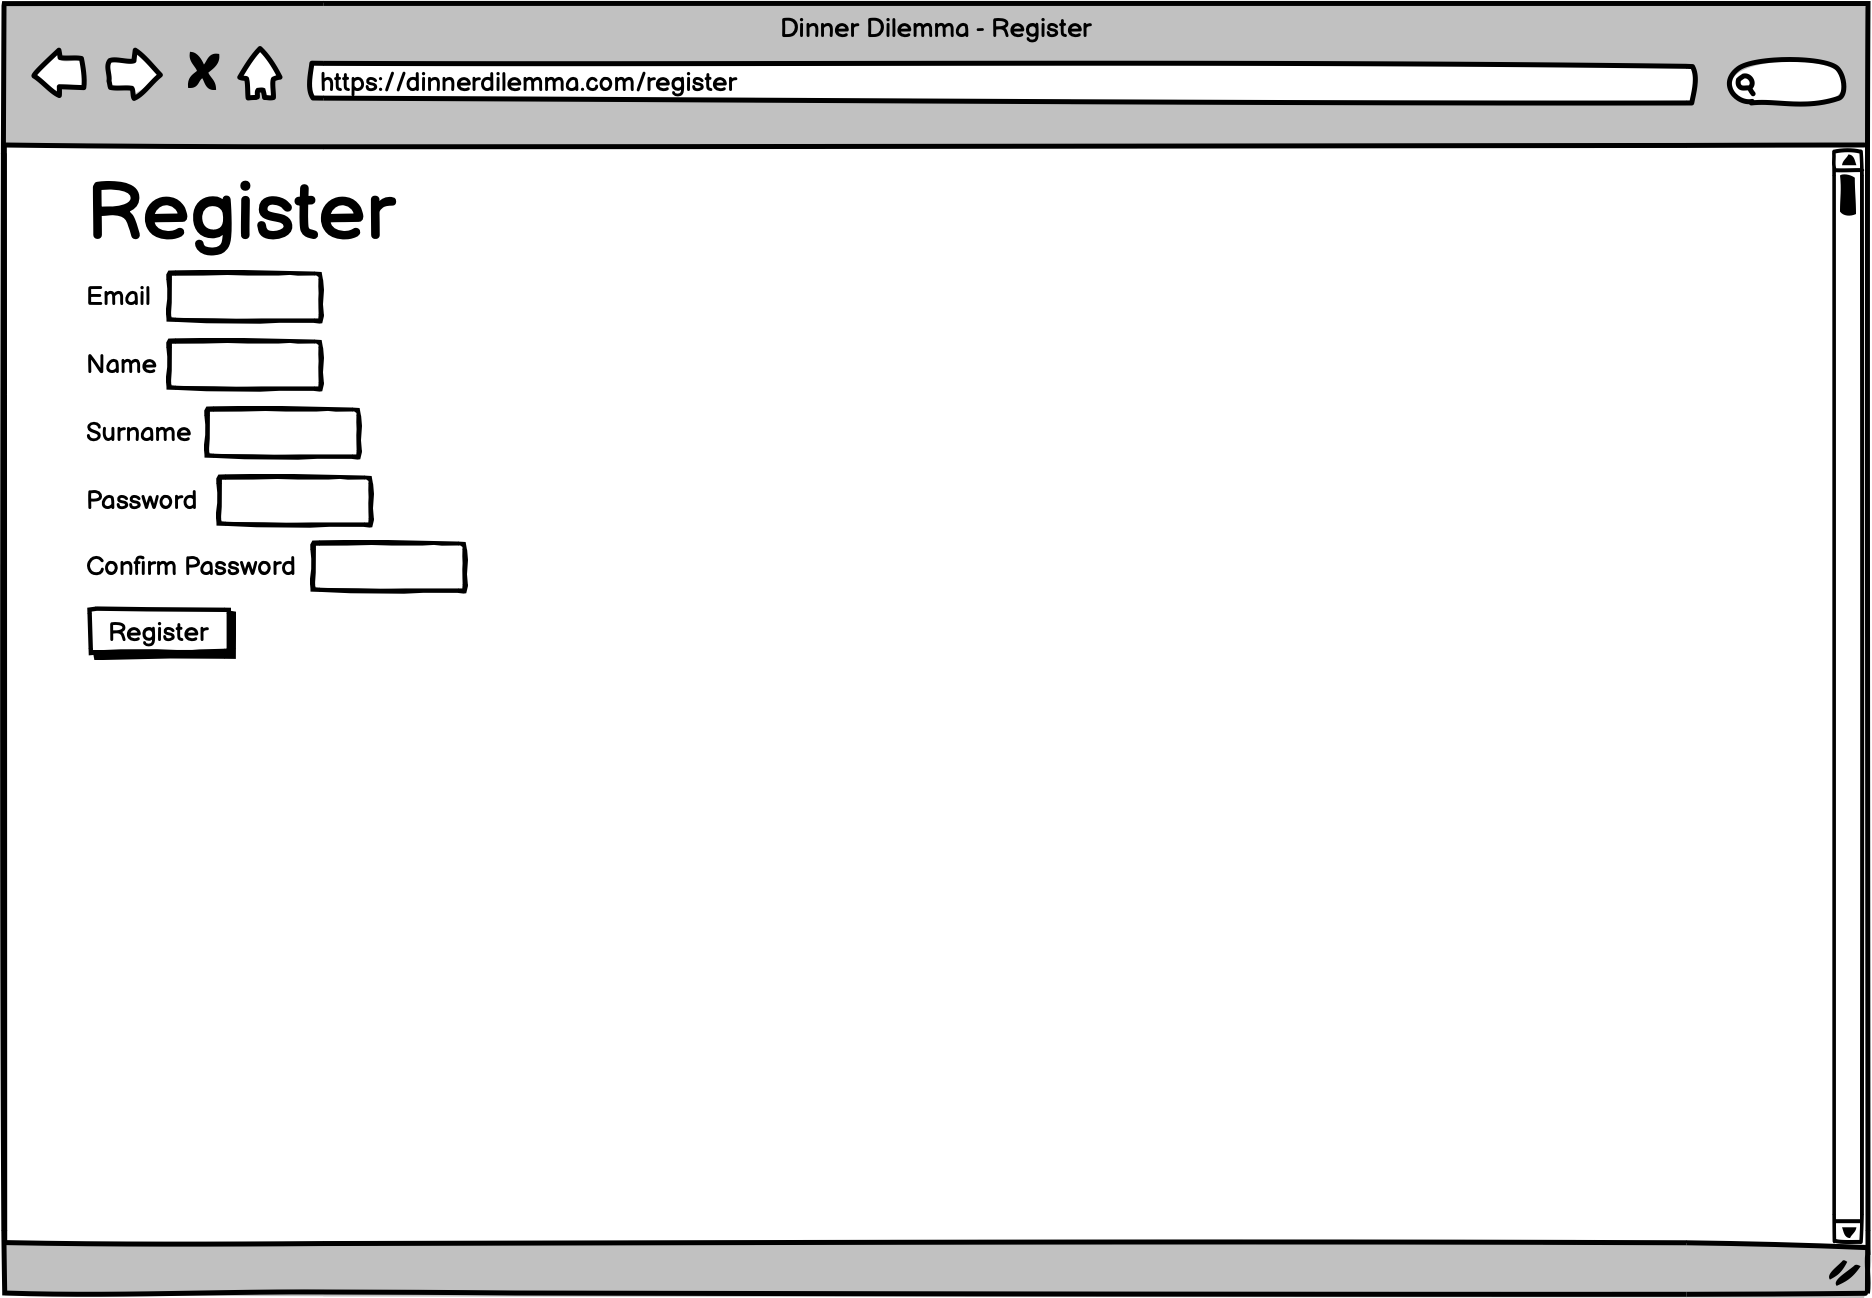
\includegraphics[width=0.75\textwidth]{images/register.png}

Page where a user can register by inputting e-mail, name, surname and password (there is also a text field to confirm the password). All checks on the input data are done to catch eventual errors and avoid duplicate emails. The id of the user is generated and the password gets hashed using SHA256. With this registration form only users of type "user" can be registrated, while "admin" users are created manually by the owners of the website. In both cases an email is sent to the registered email with a code to verify the account and the user is prompted a text field in which he needs to insert the just received code. Without this step the registration process is not completed and the user cannot login.
At the moment in this page, for test purposes only, there is a dropdown menu to choose the role of the user, so it is possible to create an admin.


\subsection{Login}
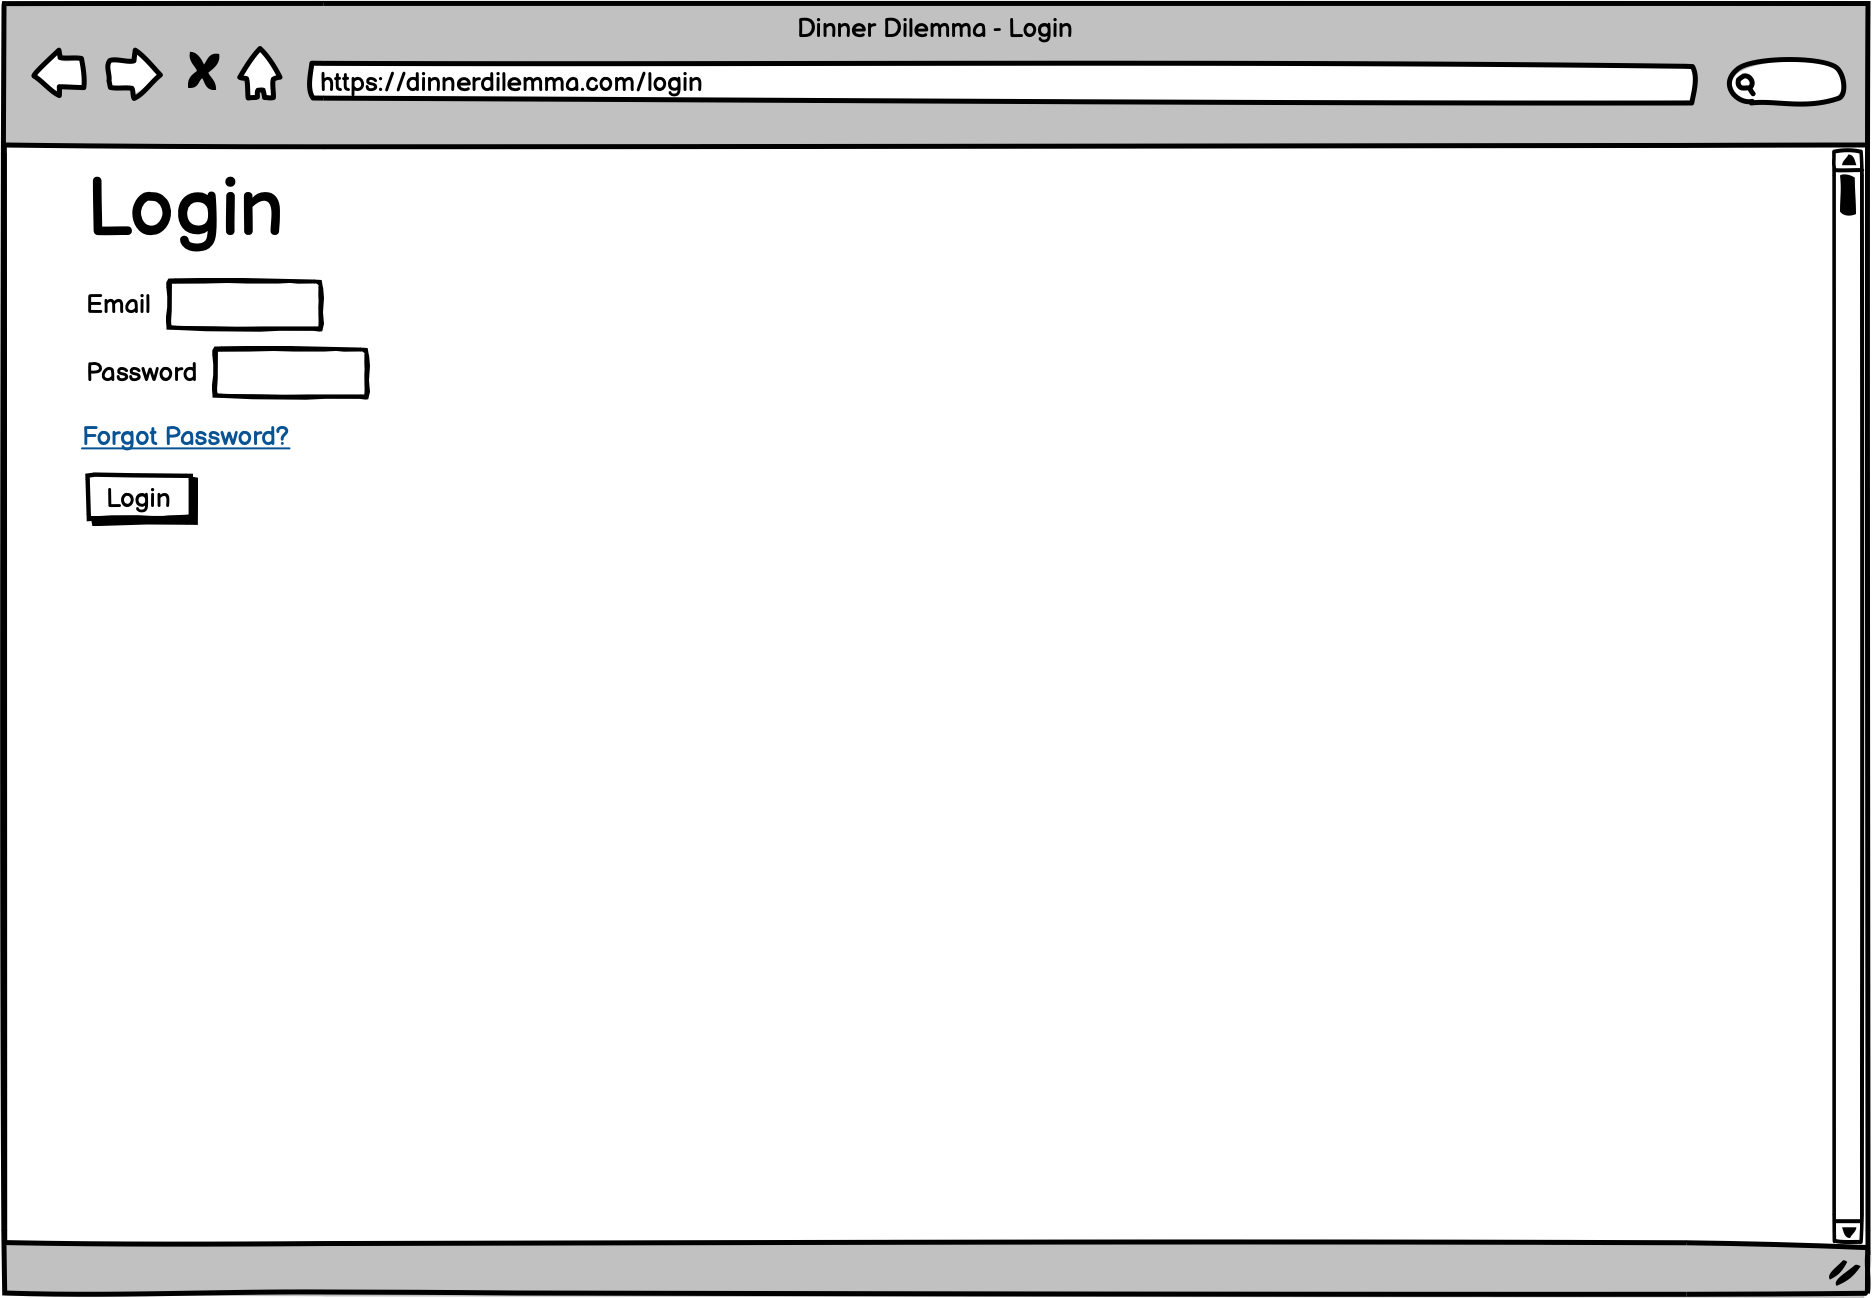
\includegraphics[width=0.75\textwidth]{images/login.png}

Simple login form where the user inputs his email and his password and, if correct, logs in and gets redirected to the home page. If the user has been banned, a popup will inform the user of his ban and he will not be able to login.\\
 An HTTP session is created so the status of the logged user is kept during the navigation on the website.\\
 There is also an option called "Forgot Password?" that, similarly to the registration flow, sends an email to the user with a code that he needs to verify to enter a page in which he can change its password.

\subsection{Verify Code}
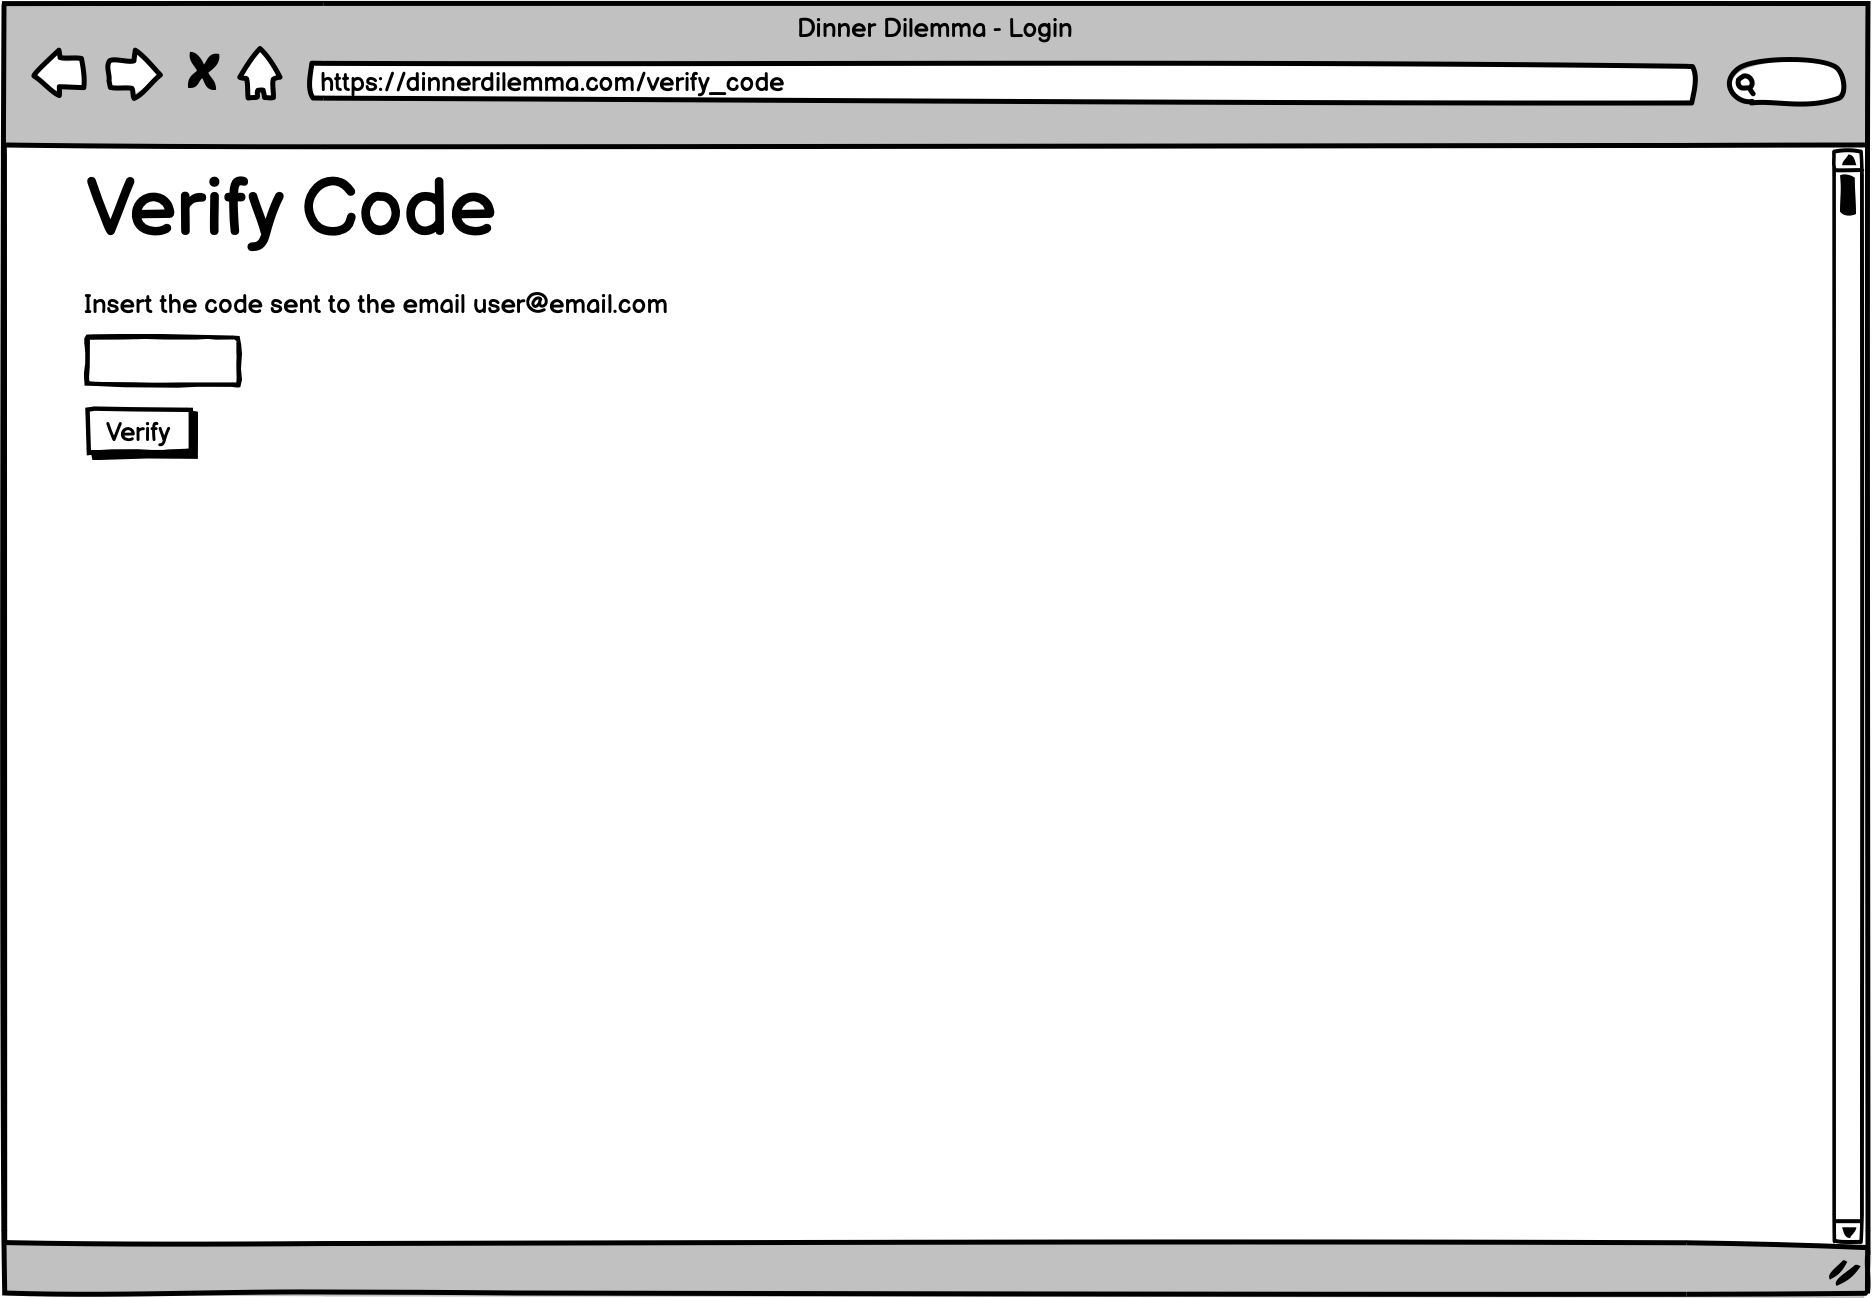
\includegraphics[width=0.75\textwidth]{images/verifycode.png}

The just mentioned page used to verify the code received via email during registration or during the forgot password process.

\subsection{Home}
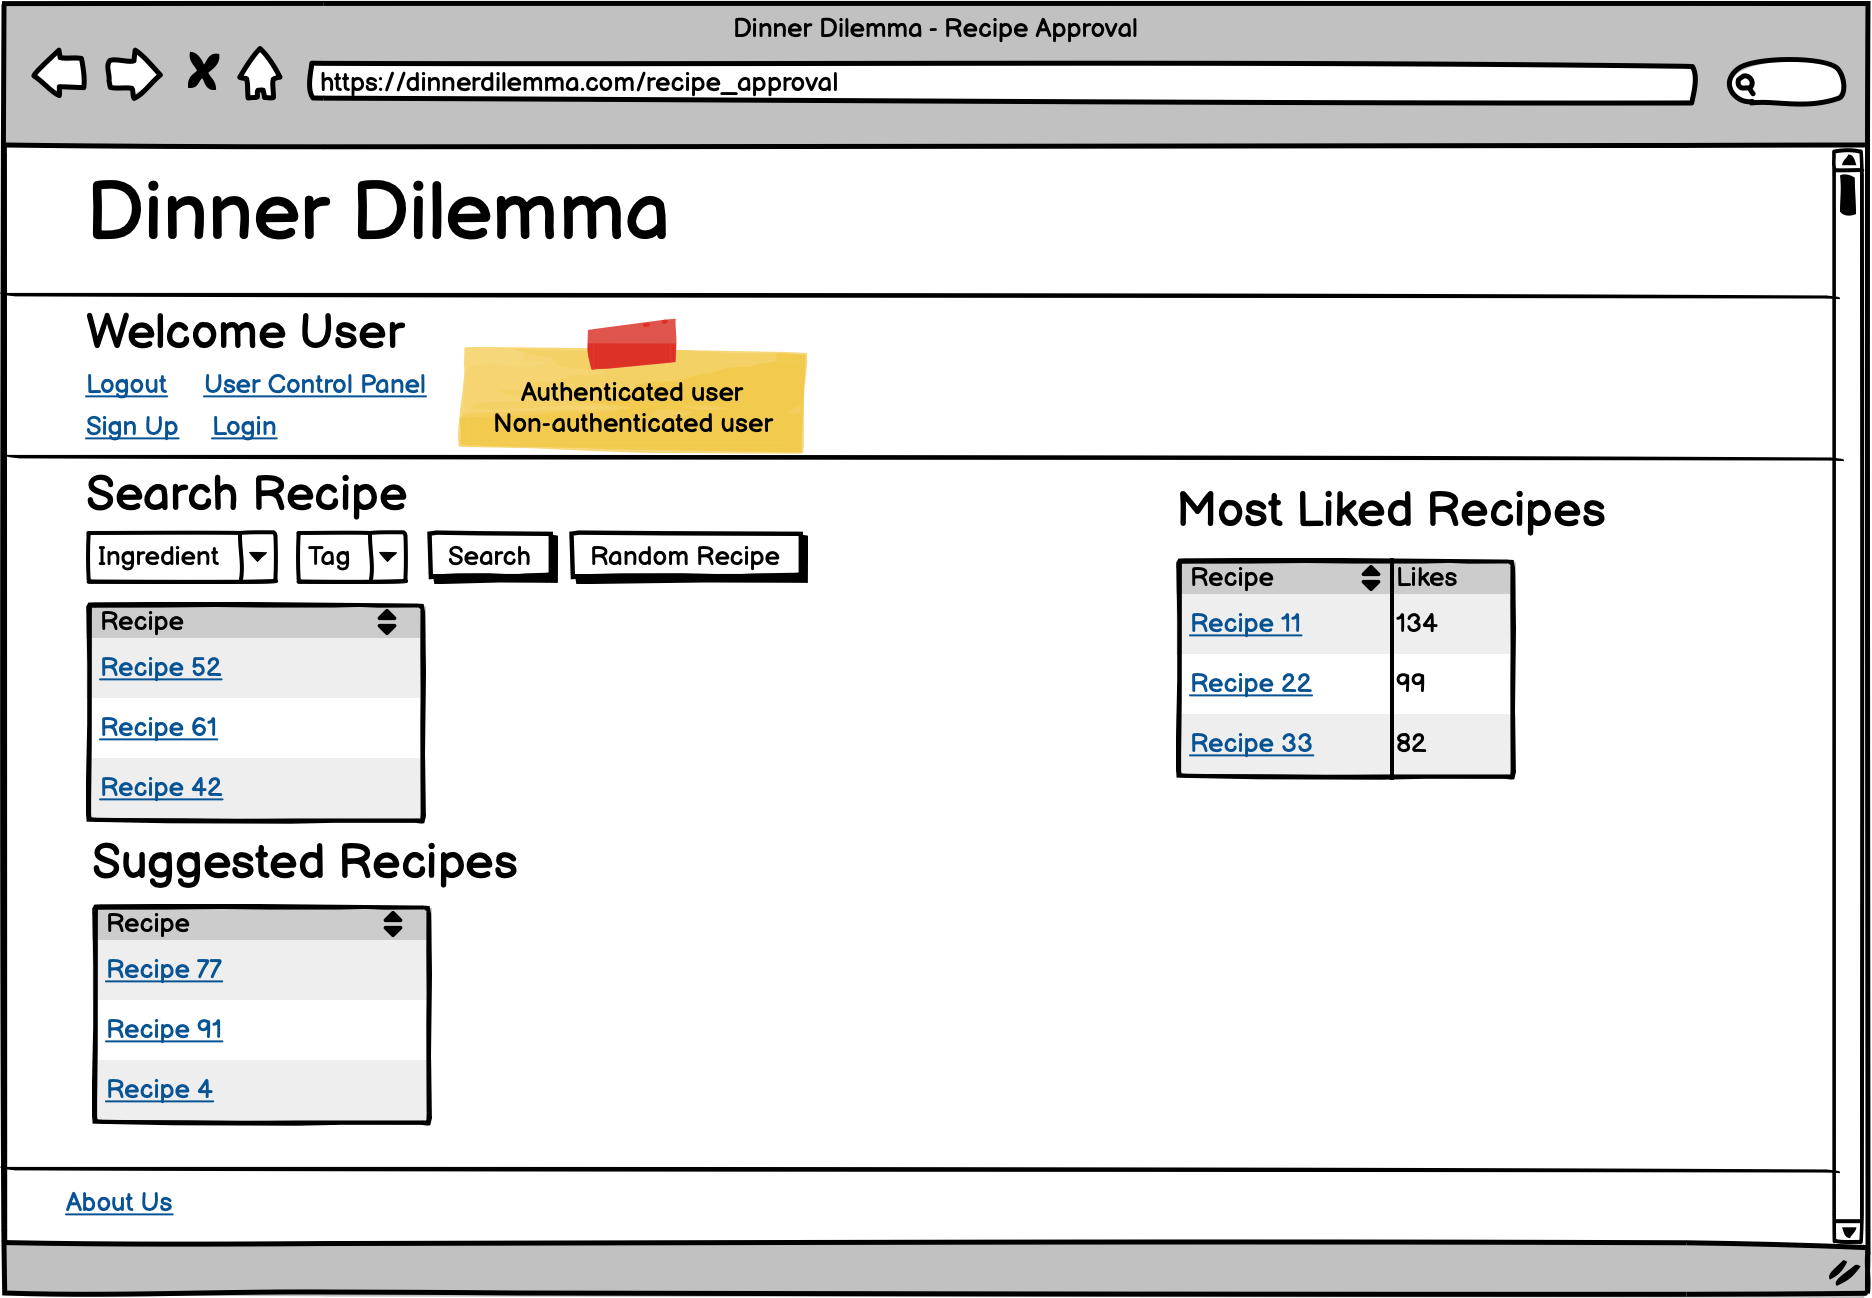
\includegraphics[width=0.75\textwidth]{images/home.png}

The home page of the website: here the user can find links to login and registration (if not already logged in) and logout (if already logged in).\\
If the user is logged in there is also a link for the user control panel page.\\
In the middle of the page the main functionality of the web app is presented (it can be accessed by everyone, even non-authenticated users): with a dropdown menu the user can choose from a list of ingredients and also from a list of tags and search recipes that use them. The result of the search is a list of recipes presented below the drop down menu and below some suggested recipies with similar ingredients appear.\\
On the right there is also a list with the most liked recipes of the website.\\
For both the two lists, the user can click on each recipe and get redirected to the related recipe details page.\\
Finally, a button inspired by Google's "I'm Feeling Lucky" that opens the details page of a random recipe is presented.\\
In the footer of the page, there is a link to the "About Us" page.



\subsection{User Control Panel}
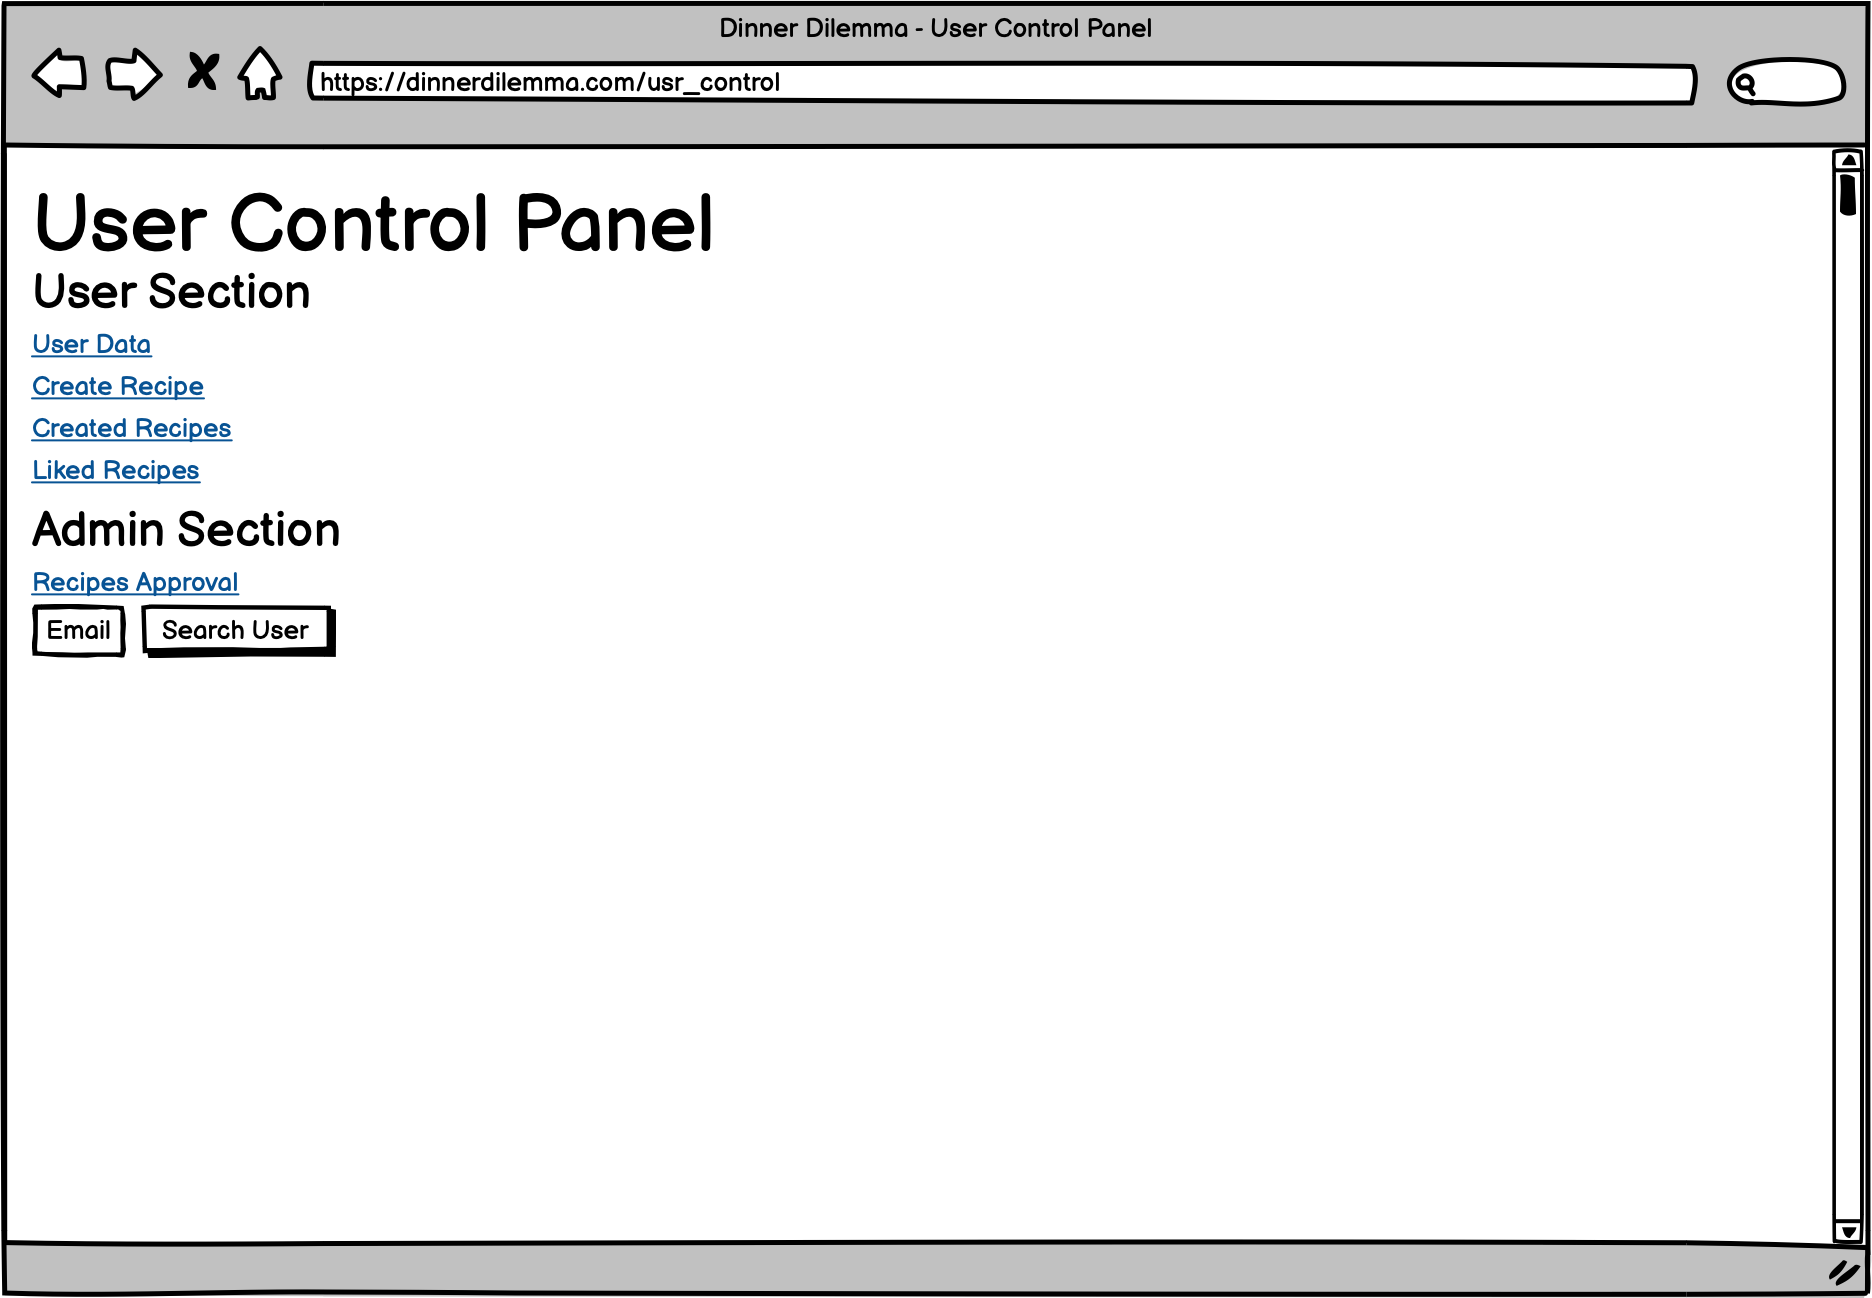
\includegraphics[width=0.75\textwidth]{images/usercontrolpanel.png}

The user control panel, accessible only by logged users, contains the link for the other pages: user data, create recipe, created recipes and liked recipes. For users of type admins, there are two links for recipes approval and recover/remove page and a text input where the admin can insert a user email and go to the search user page.
At the bottom of the page, at the moment, for test purposes only, there is a link to the log of the web app.

\subsection{User Data}
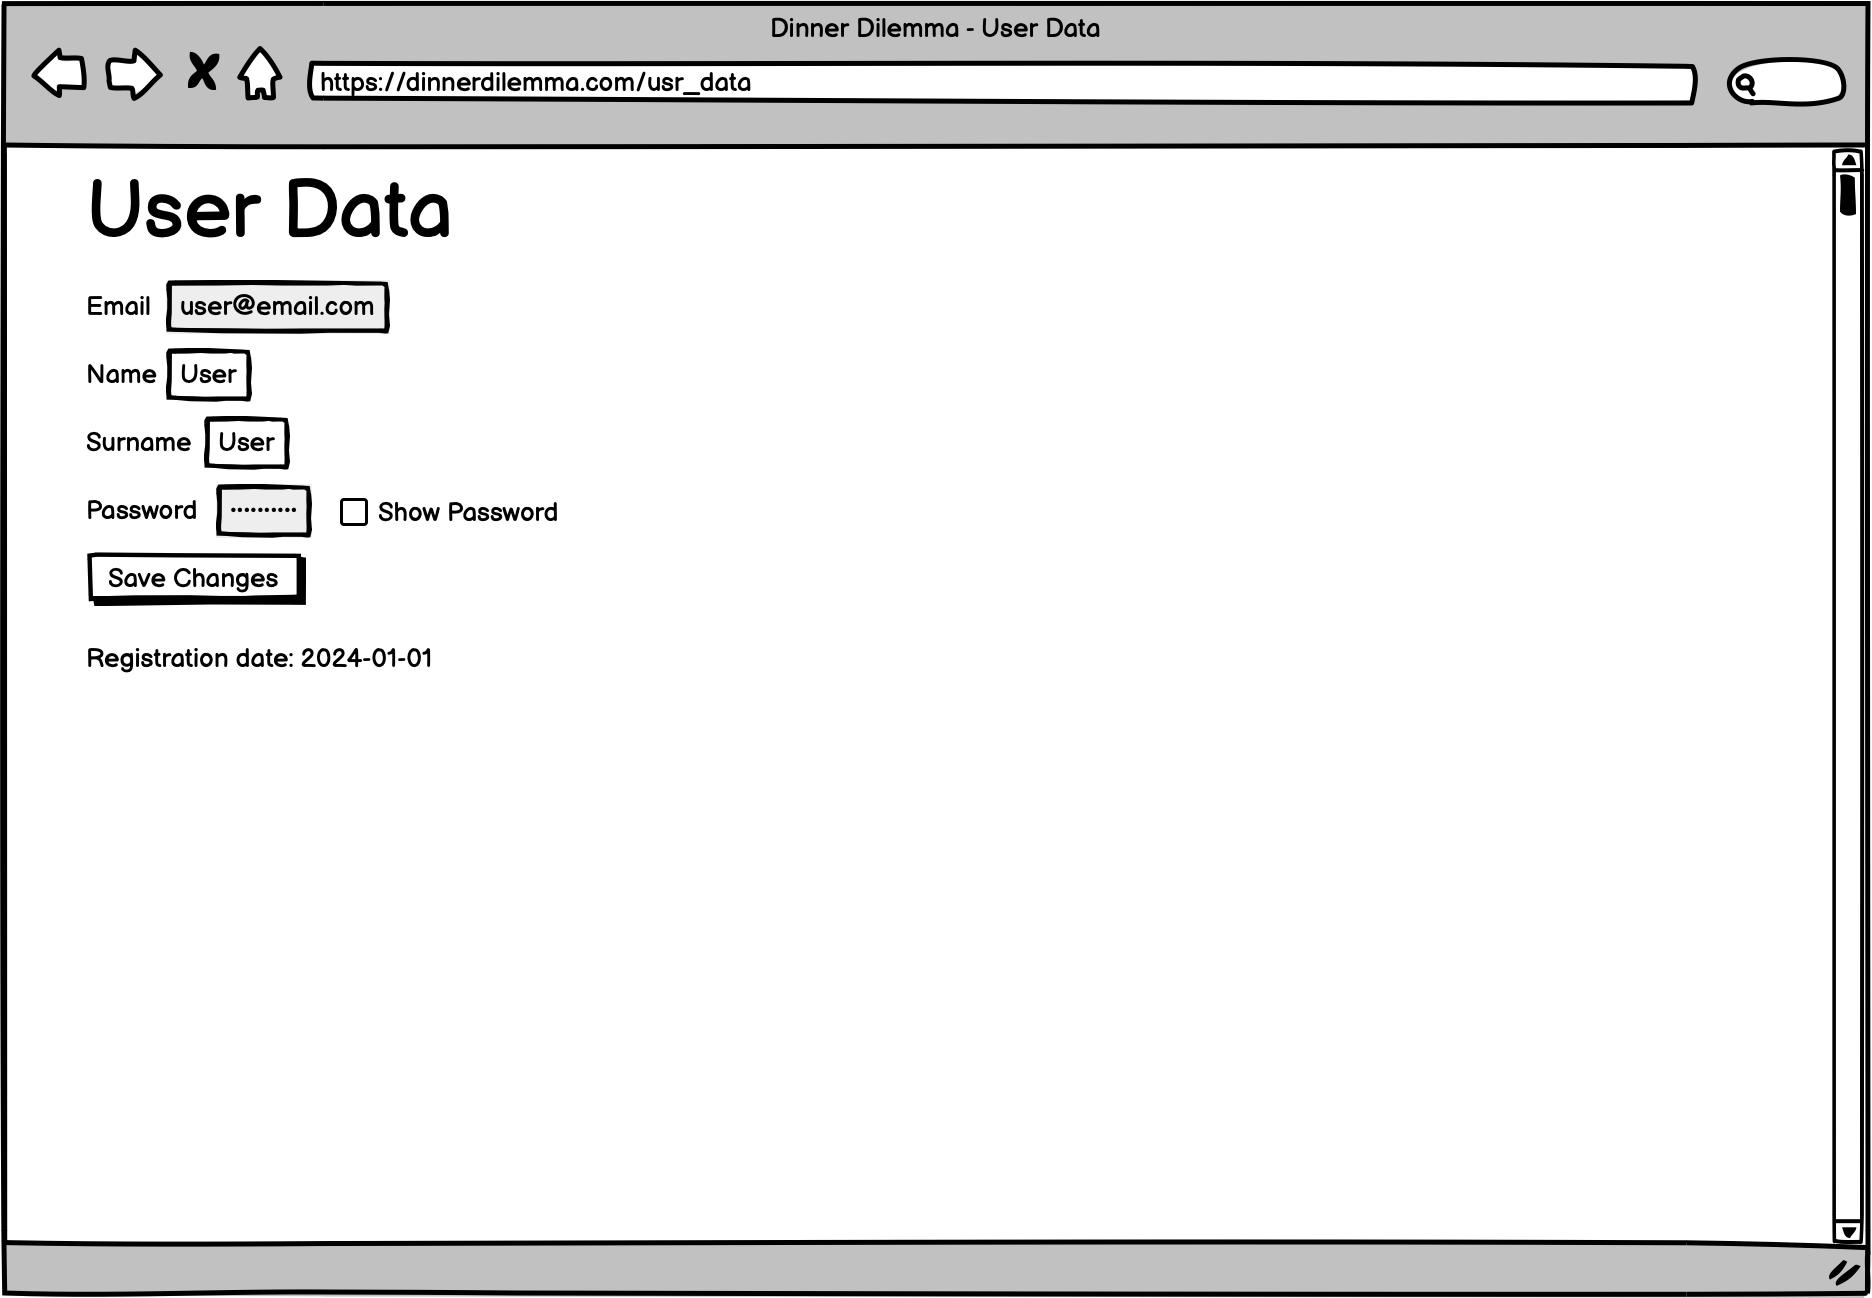
\includegraphics[width=0.75\textwidth]{images/userdata.png}

This page shows the logged user its informations inserted at registration.\\ Here the user can change its name and surname.

\subsection{Recipe}
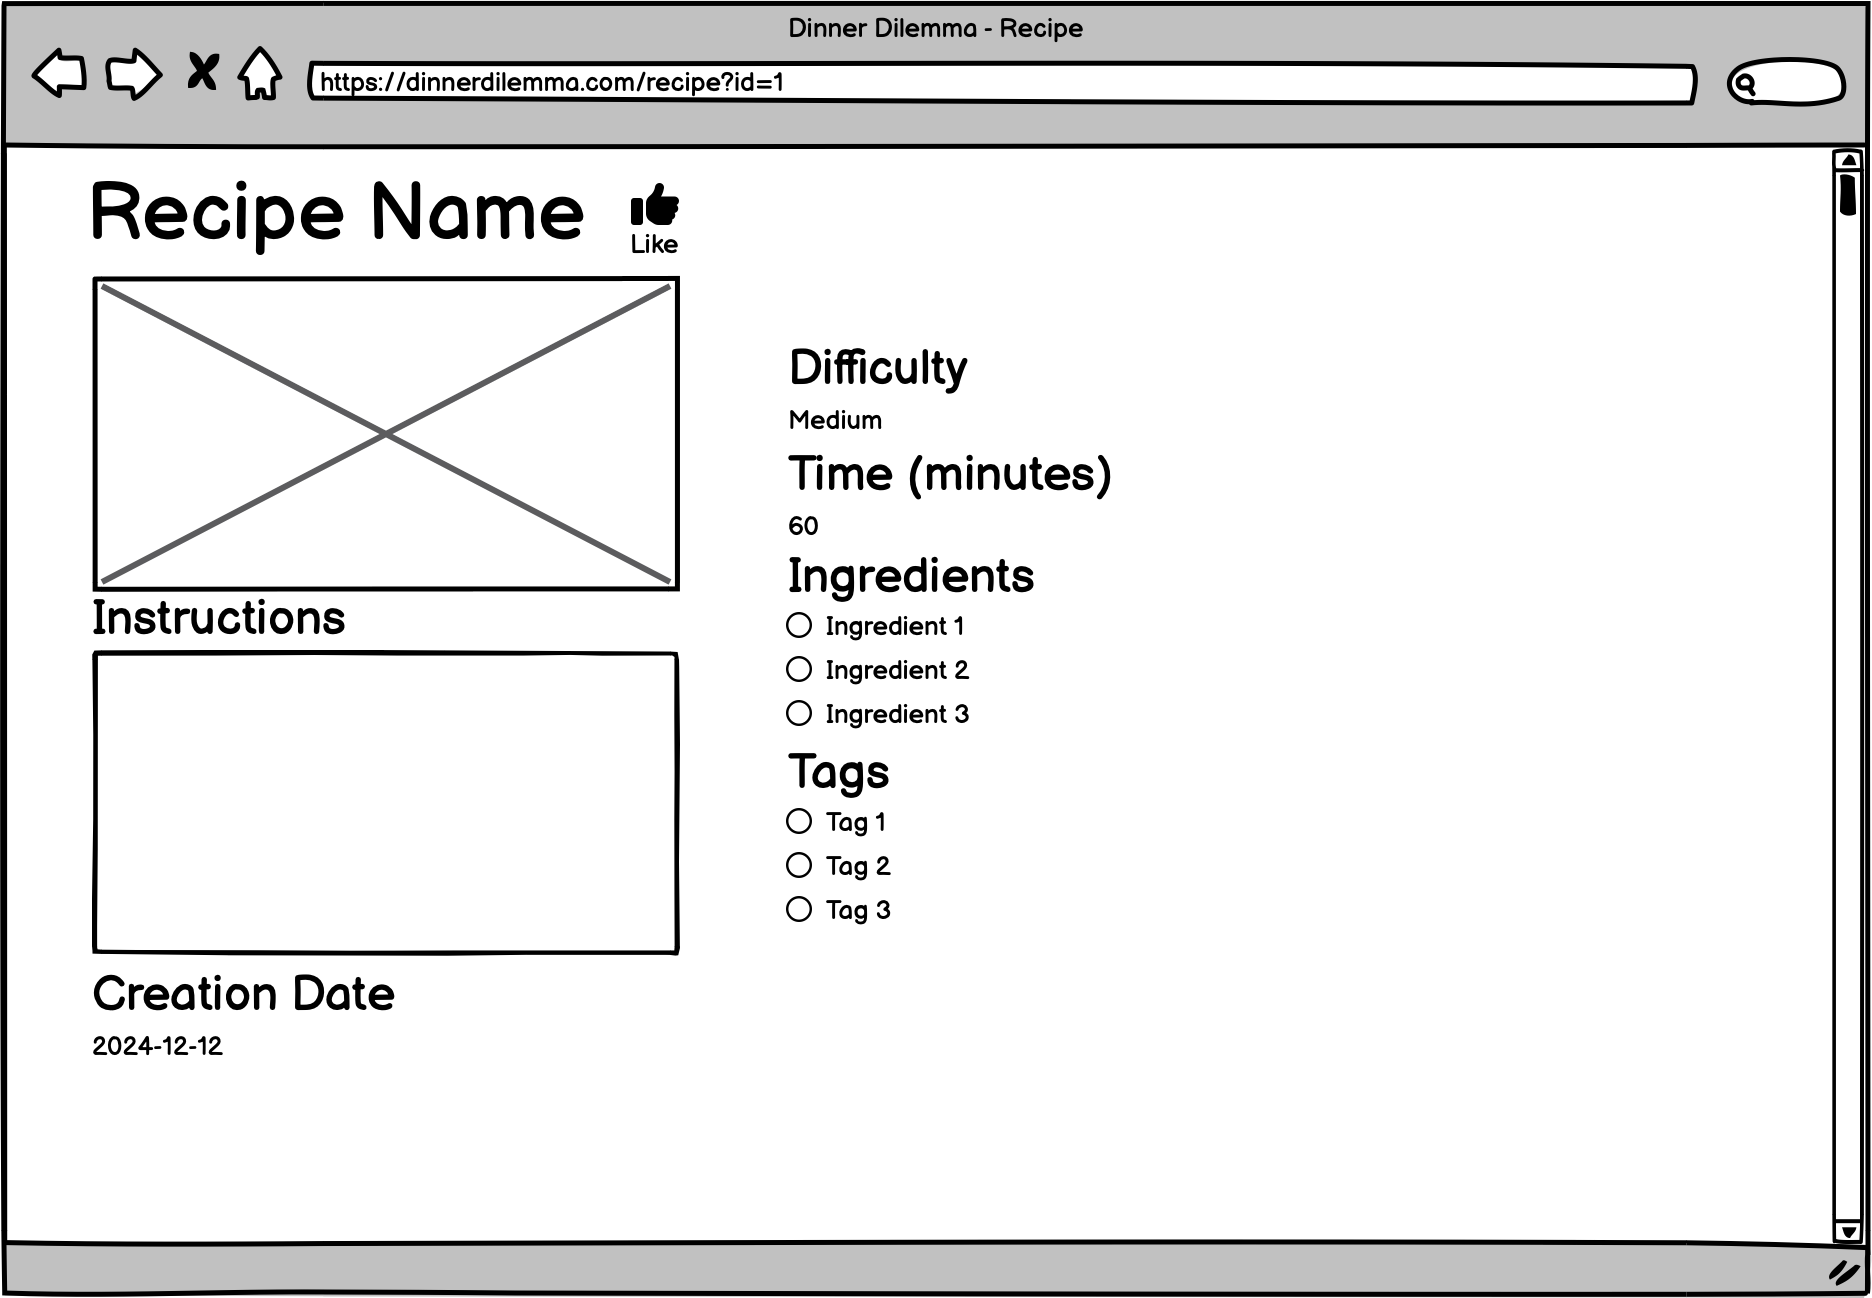
\includegraphics[width=0.75\textwidth]{images/recipe.png}

The page that shows the details of a specific recipe: the thumbnail image, the name, the description/preparation, the time required (in minutes), the name and surname of the user that inserted it, the difficulty, the ingredients, the tags and the number of likes on the recipe. Only for logged users, there is a button to like/unlike the recipe.

\subsection{Create Recipe}
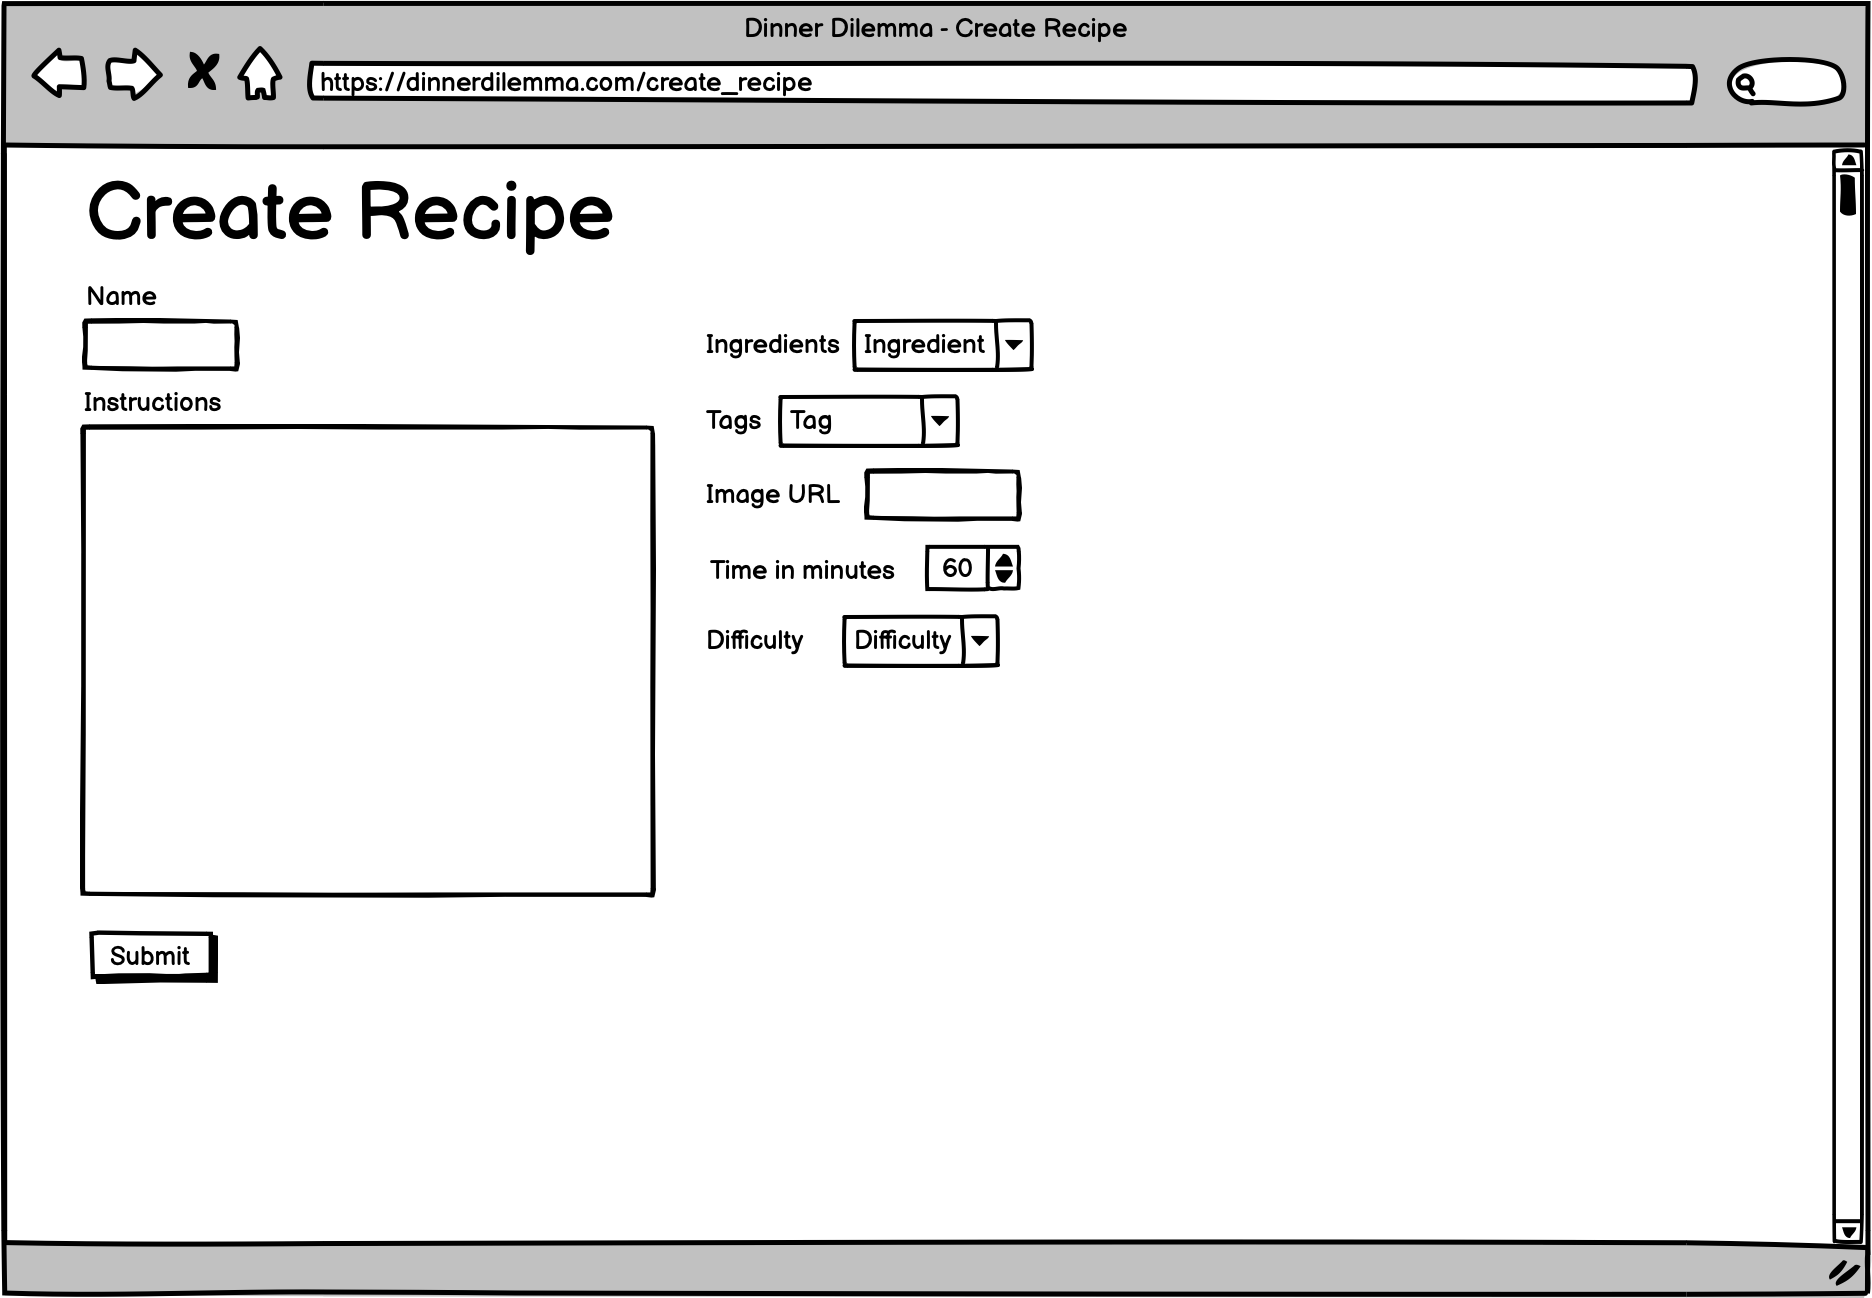
\includegraphics[width=0.75\textwidth]{images/createrecipe.png}

This form, only accessible by logged users, is used to create a recipe that once submitted, is sent to be approved by an admin. The page contains inputs for name, description, url of the thumbnail image, difficulty level and time for preparation (in minutes), a drop down menu to add the ingredients and one for the tags.

\subsection{Created Recipes}
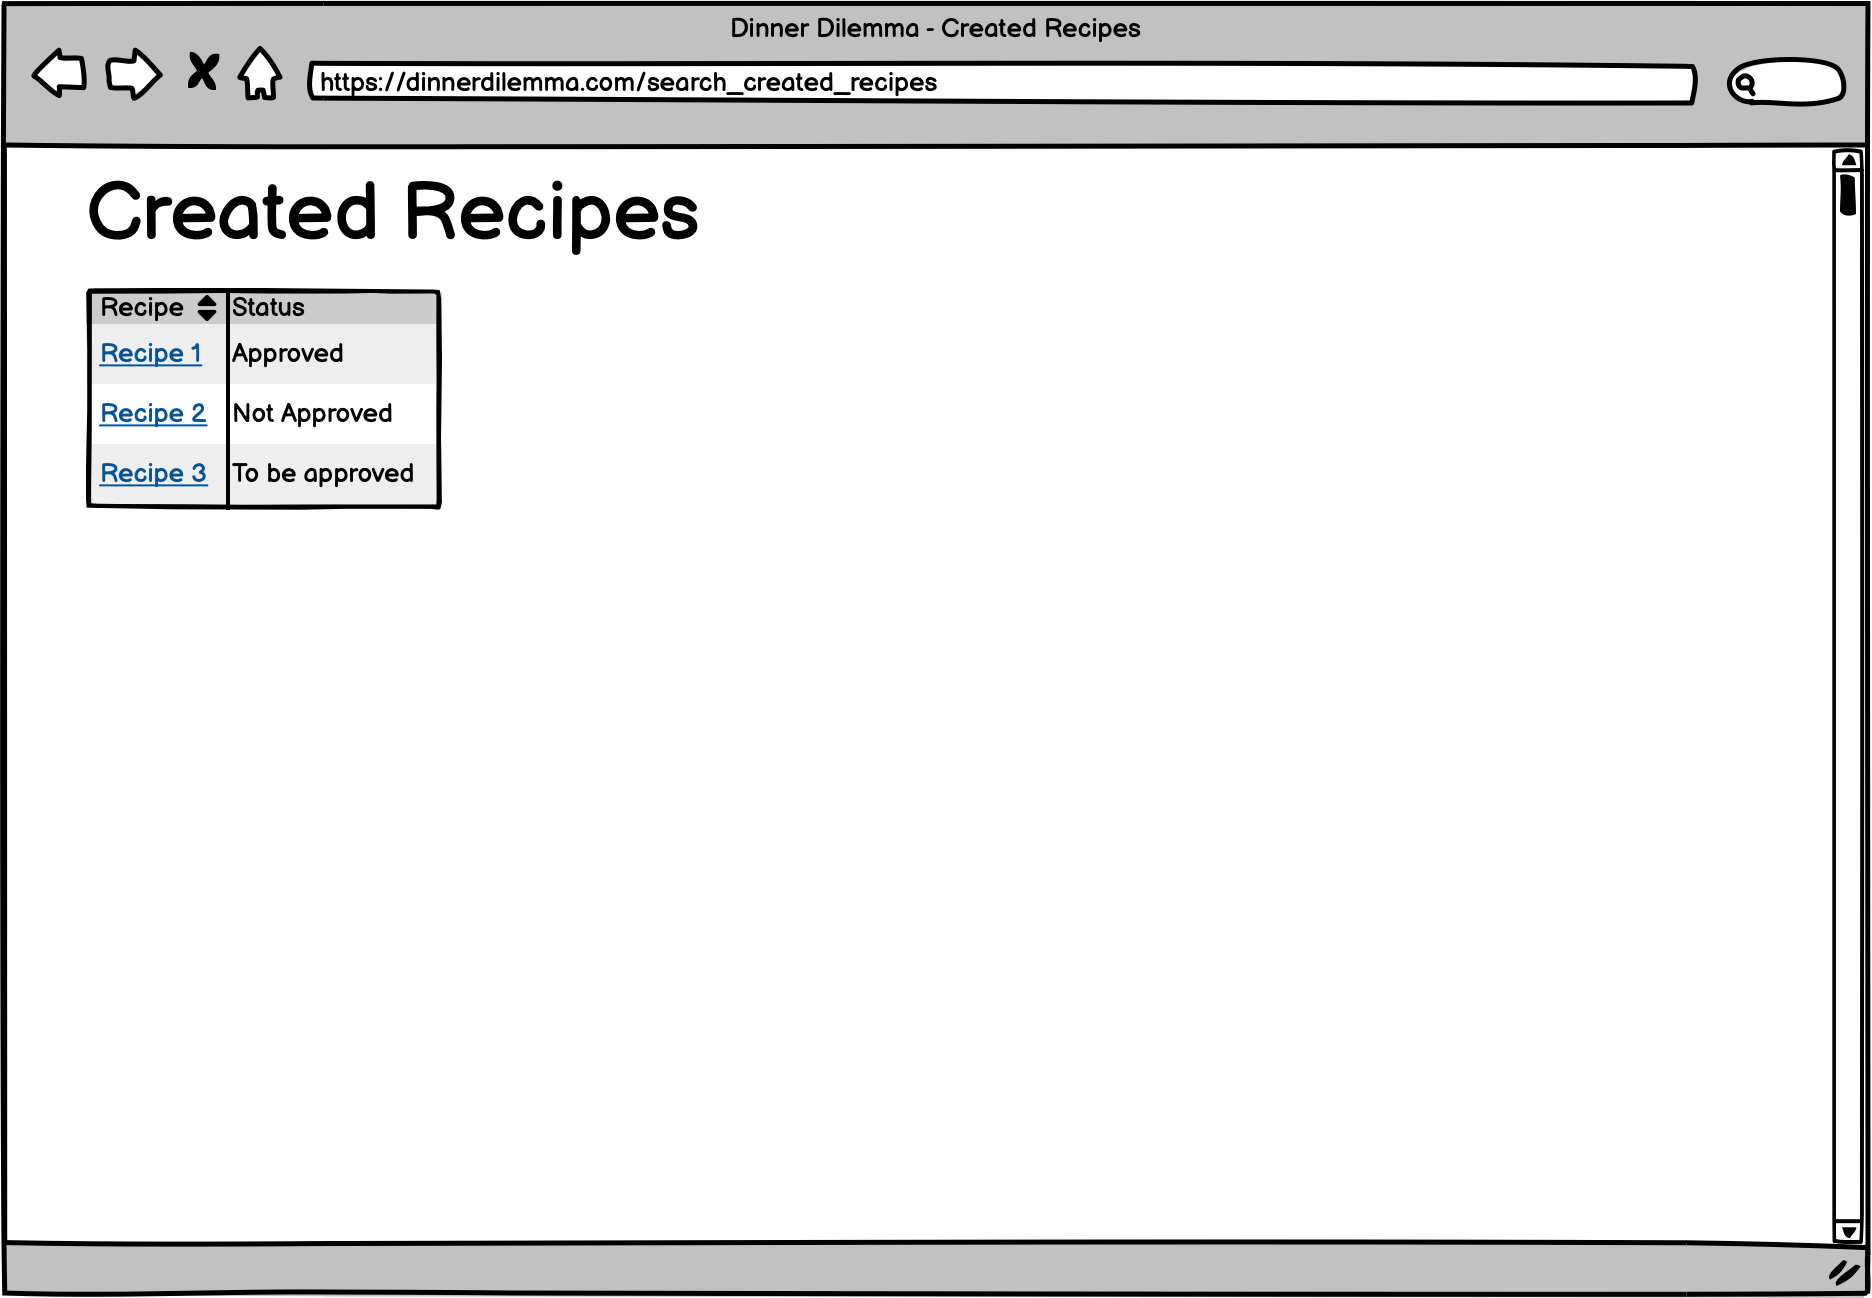
\includegraphics[width=0.75\textwidth]{images/createdrecipes.png}

In this page the logged user can see the list of the recipes he created, along with the status of each one to find out if they have been approved or not. 

\subsection{Liked Recipes}
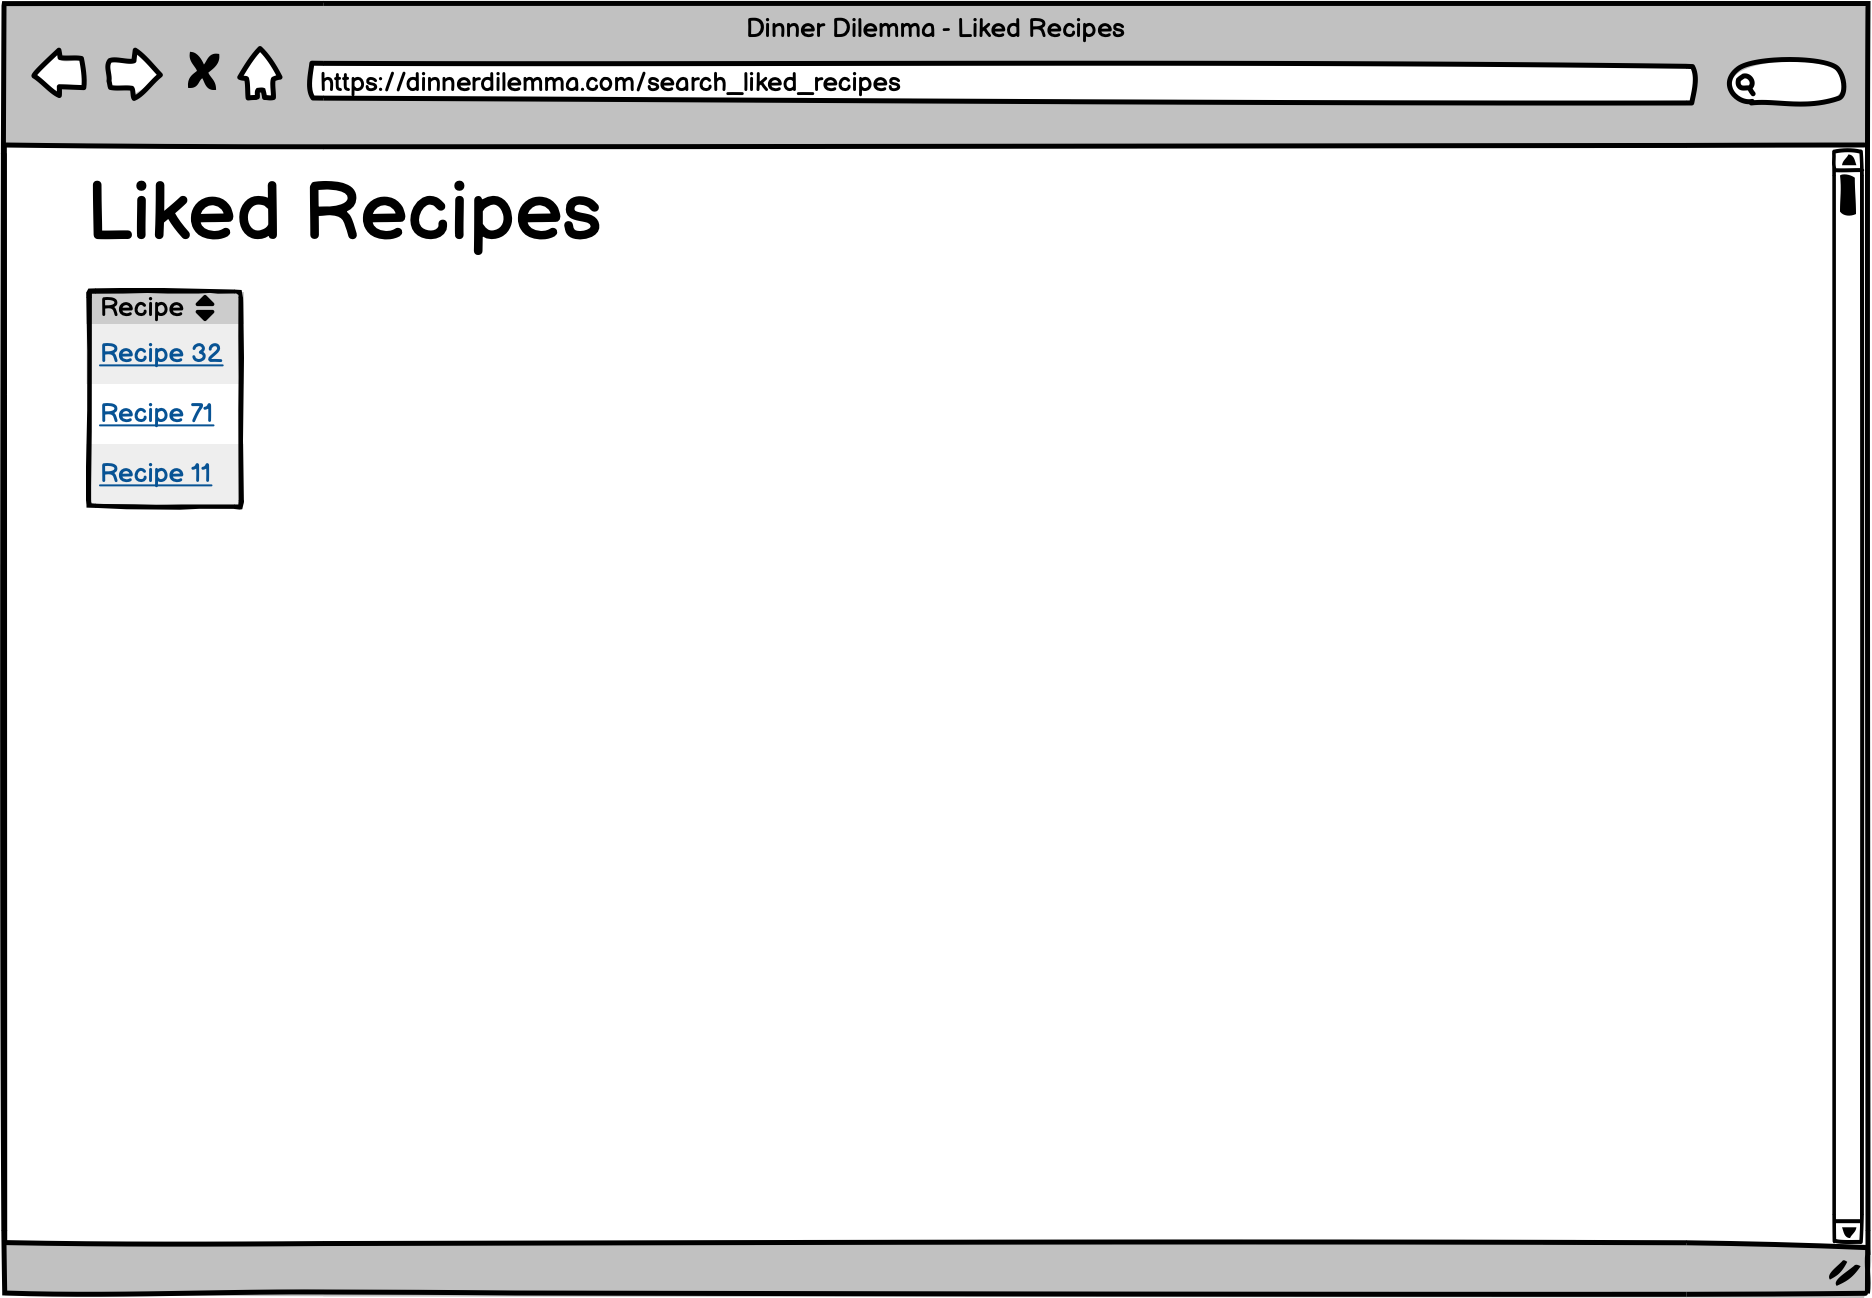
\includegraphics[width=0.75\textwidth]{images/likedrecipes.png}

A list of the recipes liked by the logged user.

\subsection{Recipies Approval}
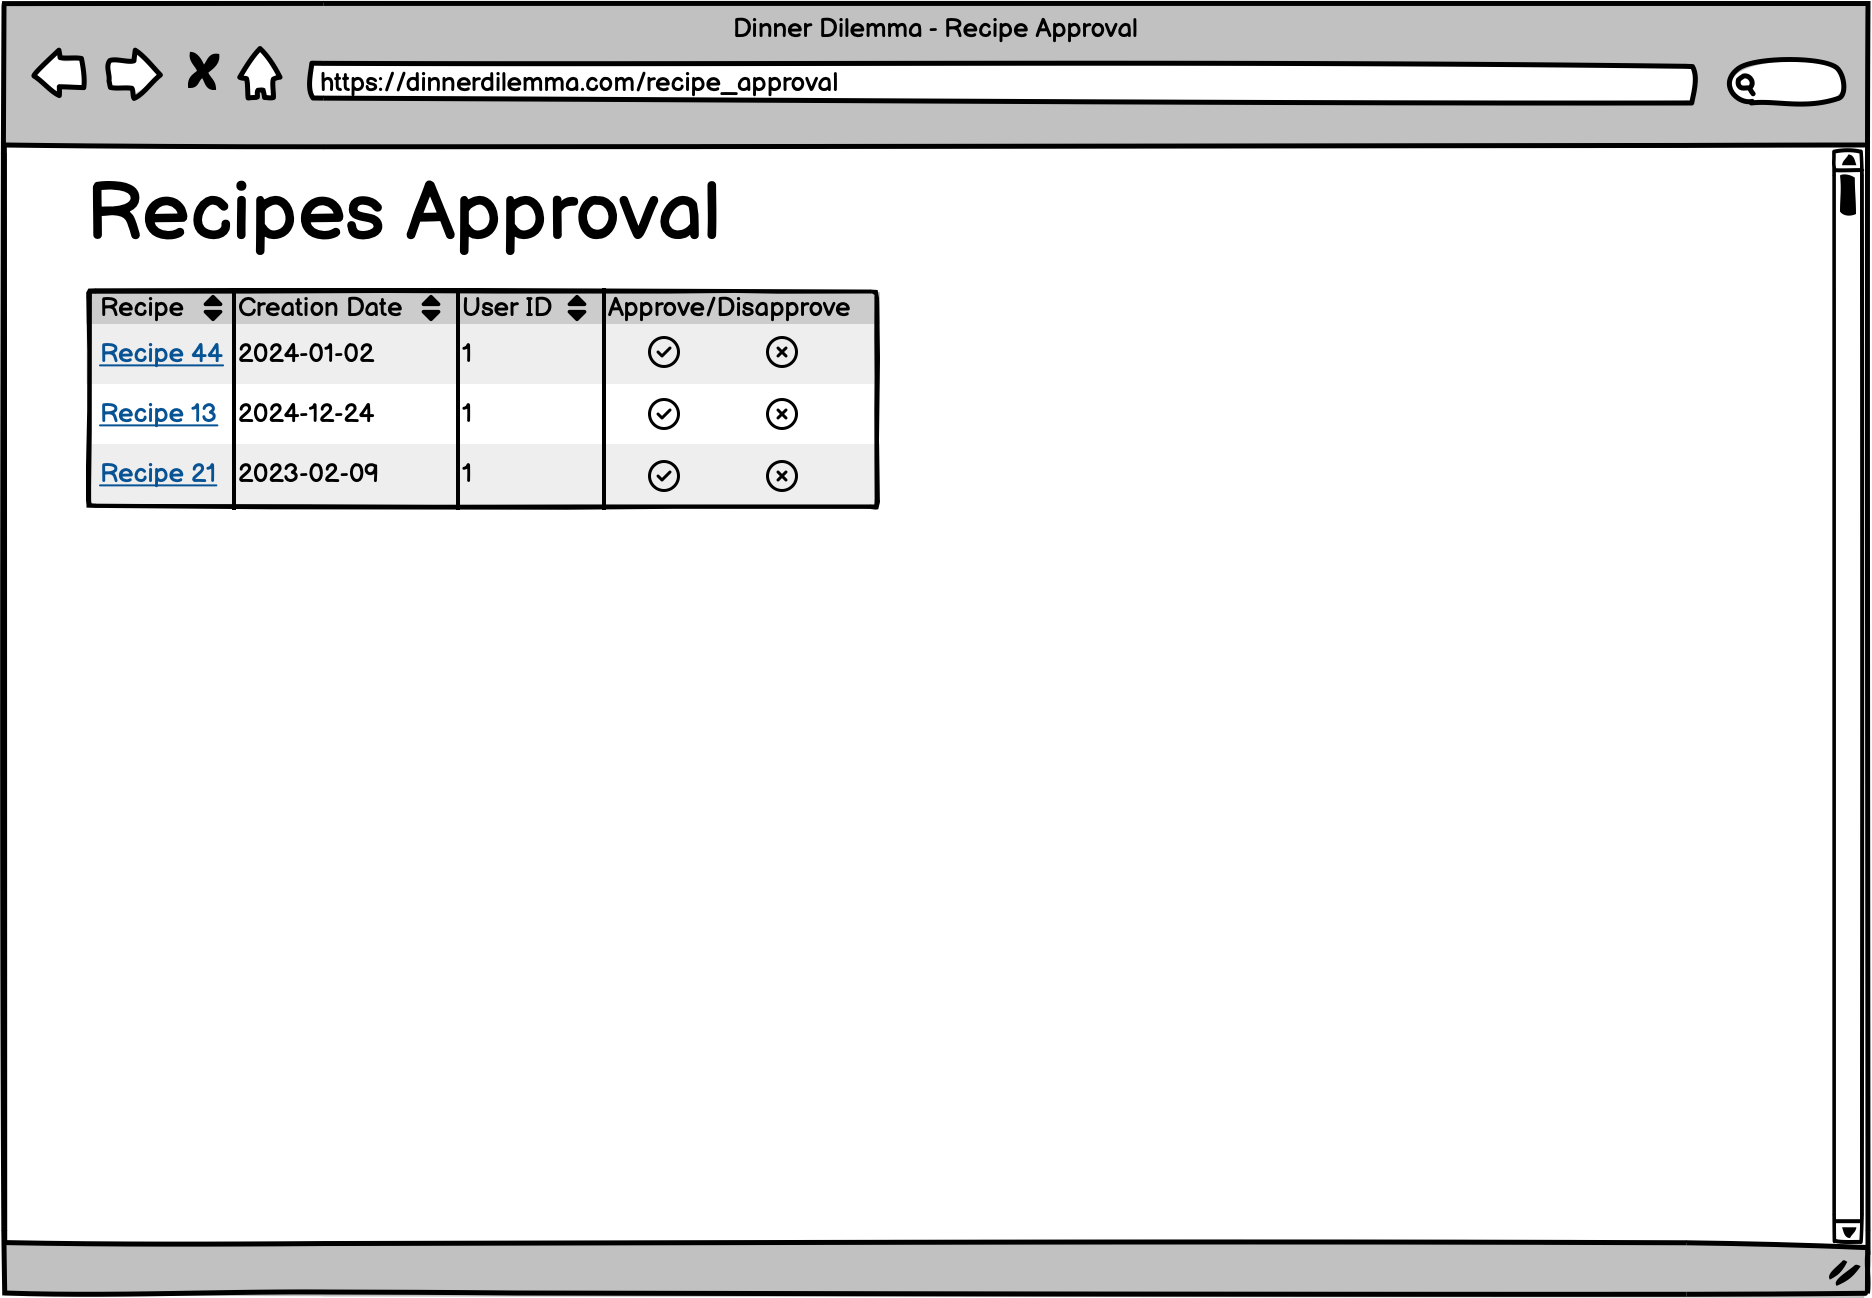
\includegraphics[width=0.75\textwidth]{images/recipesapproval.png}

A page where the logged admin can see the recipes that are waiting to be approved. He has the possibility to approve or disapprove them.


\subsection{Recipes Recover Or Removal}
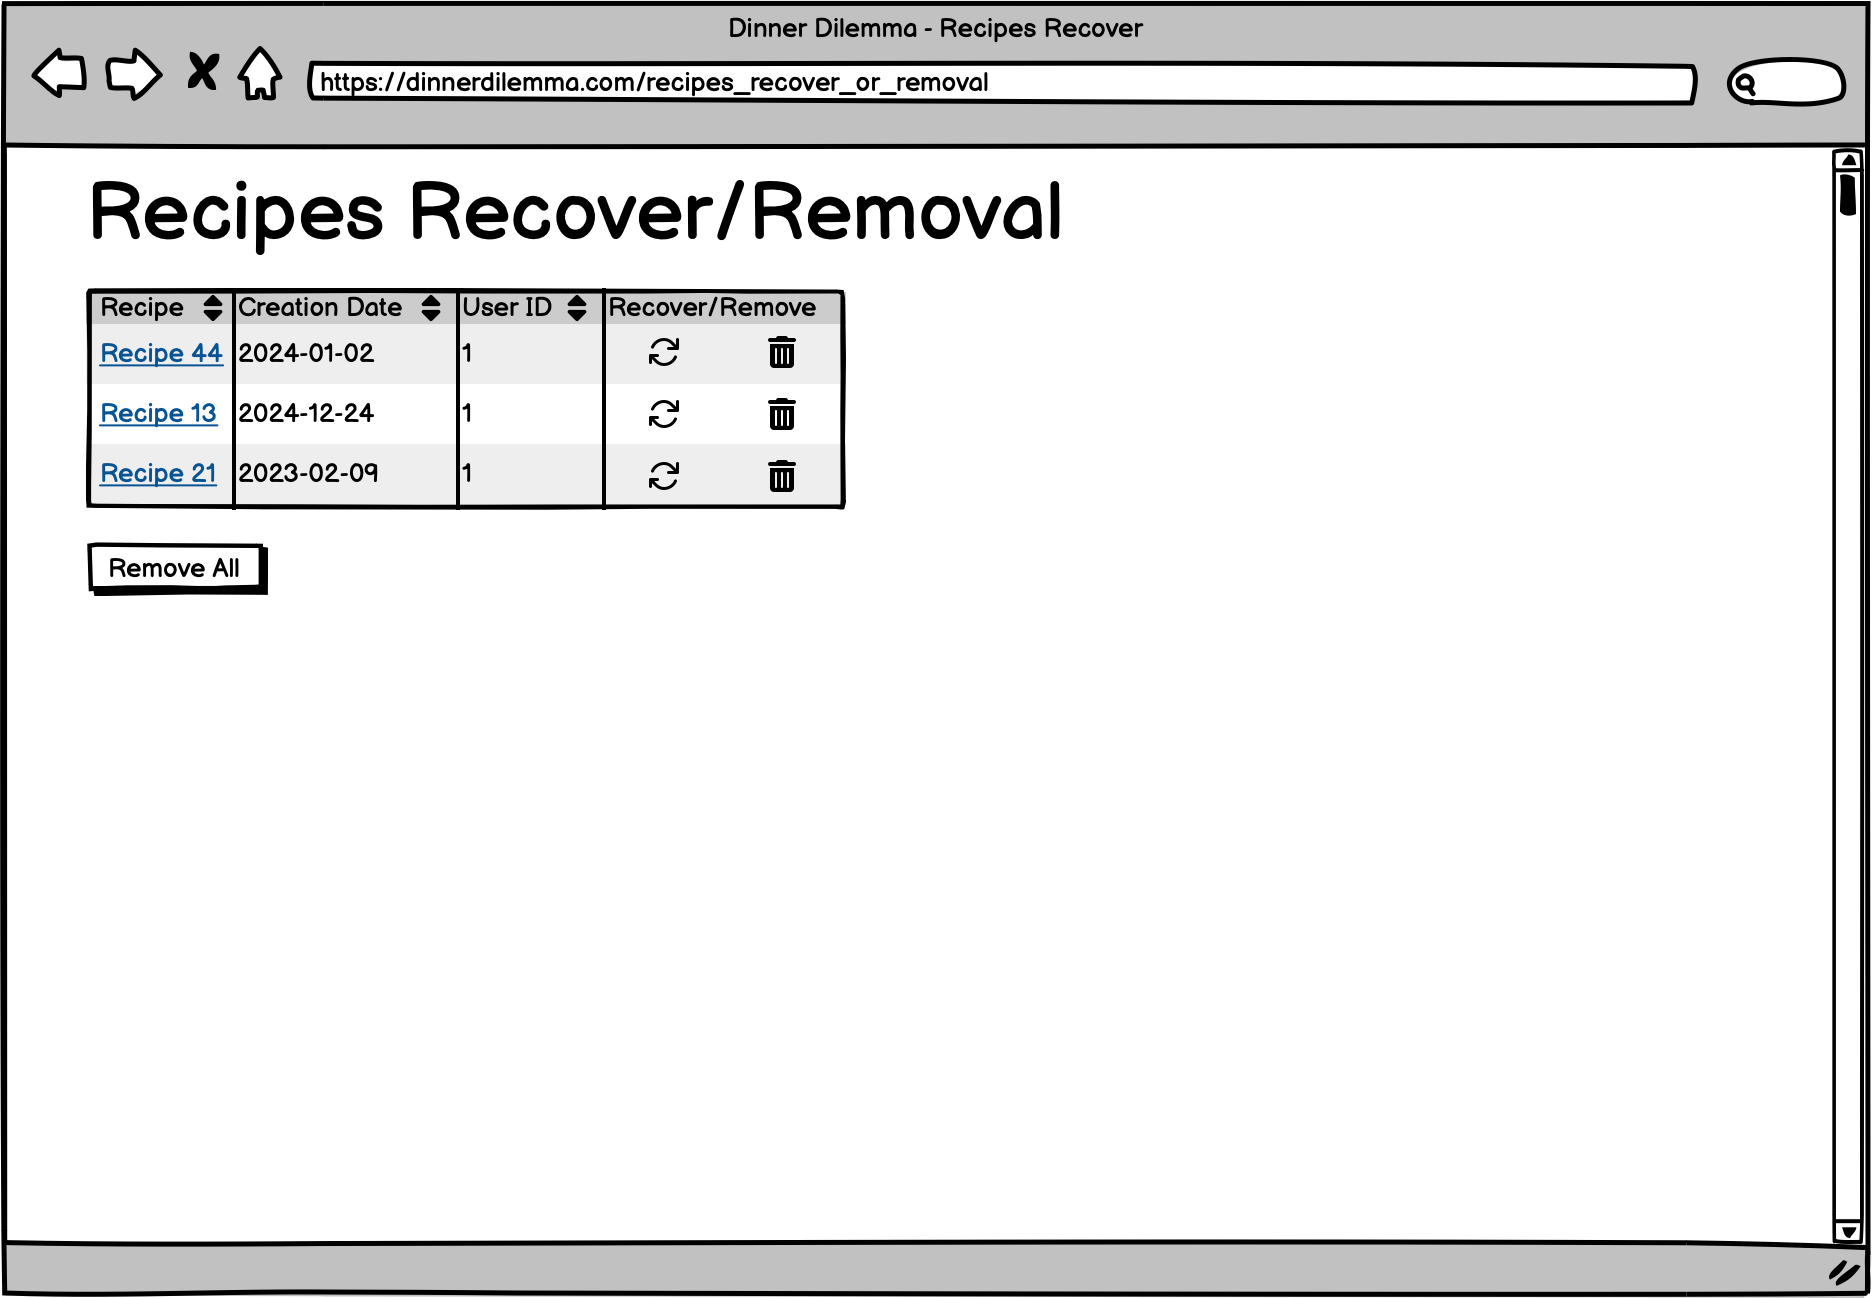
\includegraphics[width=0.75\textwidth]{images/recipesrecoverorremoval.png}

Contrary to the last cited page, here the logged admin can see the recipes that have been rejected and can decide if recover them or completely delete them from the database.
There is also a button to remove all the rejected recipes.



\subsection{Search User}
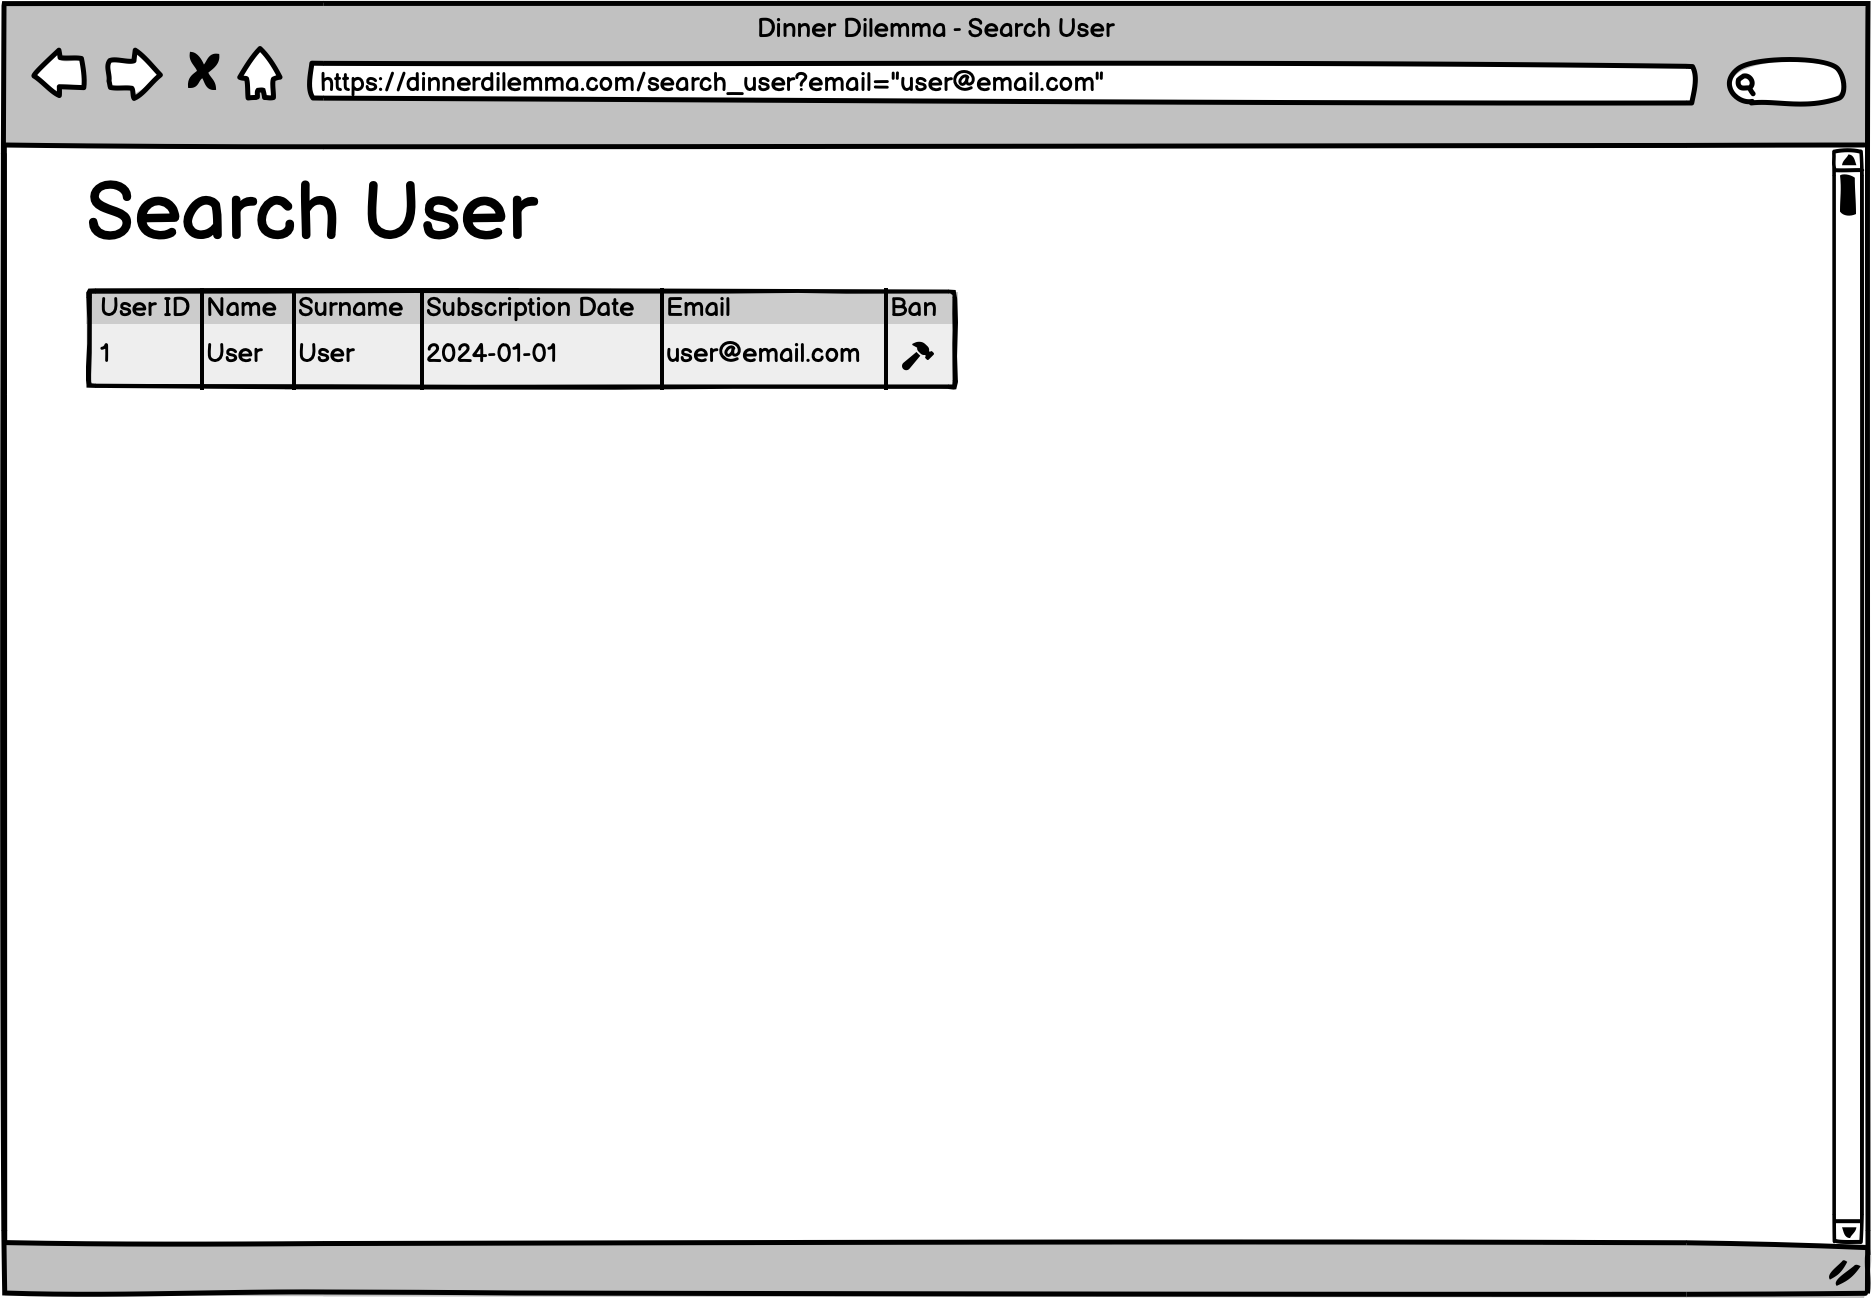
\includegraphics[width=0.75\textwidth]{images/searchuser.png}

In this page a logged admin can see the information of the user associated with the specific email inputted in the user control page. Along with this he has the possibility to ban the user.


\subsection{About Us}
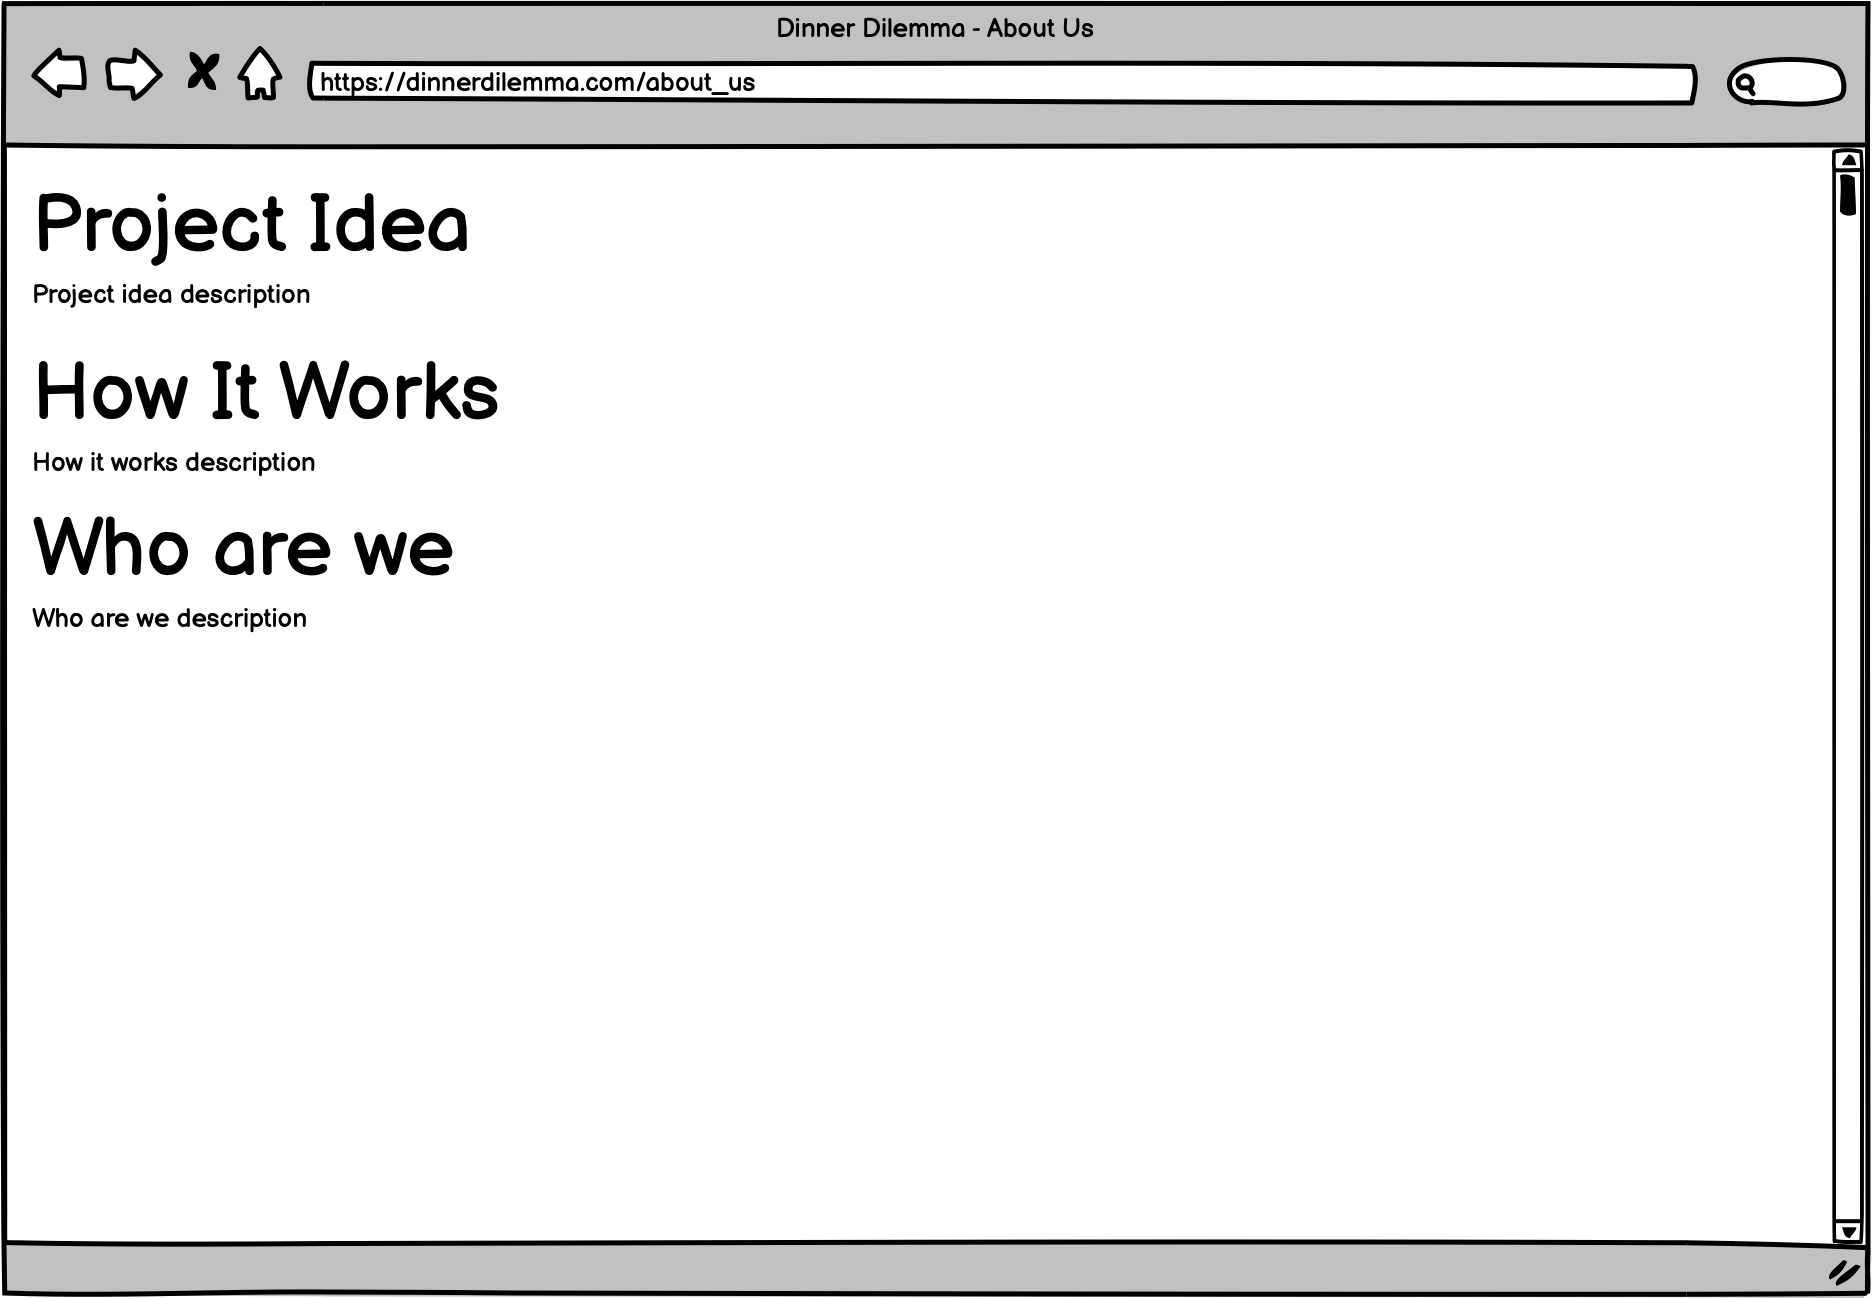
\includegraphics[width=0.75\textwidth]{images/aboutus.png}

A simple page with the description of Dinner Dilemma and a guide on how the website works. There is also a short section to list the creators of the web app.

